% Why the solid is a pyramid: every horizontal slice is a rectangle [0,1-z] x [0,2-2z].
% Rectangles at z = 0, 0.25, 0.5, 0.75 shrink toward the apex (0,0,1).
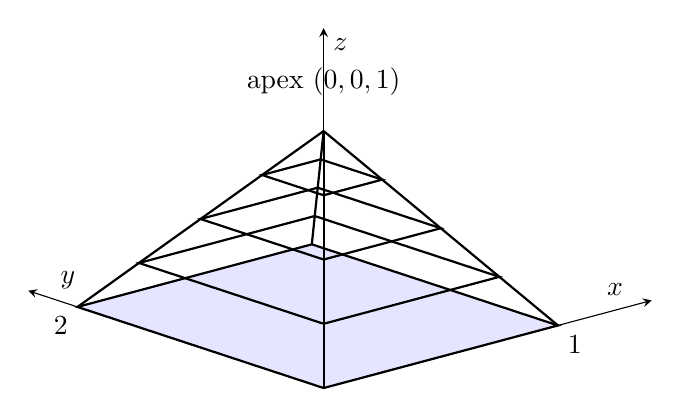
\begin{tikzpicture}
\begin{axis}[
    view={-42}{20},
    axis lines=center,
    axis line style={-stealth},
    xlabel={$x$}, ylabel={$y$}, zlabel={$z$},
    xmin=0, xmax=1.4,
    ymin=0, ymax=2.4,
    zmin=0, zmax=1.4,
    xtick=\empty, ytick=\empty, ztick=\empty,
    width=9.5cm, height=8.5cm,
    clip=false,
]
% base rectangle z=0
\addplot3[fill=blue!20, fill opacity=0.5, draw=black, thick]
    coordinates {(0,0,0) (1,0,0) (1,2,0) (0,2,0) (0,0,0)};
% slices
\addplot3[draw=black, thick] coordinates {(0,0,0.25)(0.75,0,0.25)(0.75,1.5,0.25)(0,1.5,0.25)(0,0,0.25)};
\addplot3[draw=black, thick] coordinates {(0,0,0.5) (0.5,0,0.5) (0.5,1,0.5)  (0,1,0.5) (0,0,0.5)};
\addplot3[draw=black, thick] coordinates {(0,0,0.75)(0.25,0,0.75)(0.25,0.5,0.75)(0,0.5,0.75)(0,0,0.75)};
% lateral edges to the apex
\draw[thick] (axis cs:0,0,1) -- (axis cs:1,0,0);
\draw[thick] (axis cs:0,0,1) -- (axis cs:1,2,0);
\draw[thick] (axis cs:0,0,1) -- (axis cs:0,2,0);
\draw[thick] (axis cs:0,0,1) -- (axis cs:0,0,0);
\node[above] at (axis cs:0,0,1.1) {apex $(0,0,1)$};
\node[below right] at (axis cs:1,0,0) {$1$};
\node[below left]  at (axis cs:0,2,0) {$2$};
\end{axis}
\end{tikzpicture}
